\documentclass[a4paper,14pt]{extarticle}
\usepackage{color}
\usepackage{amsmath}
\usepackage{amsthm}
\usepackage{amssymb}
\usepackage{centernot}
\usepackage{tikz}
\usepackage{caption}

\theoremstyle{definition}
\newtheorem*{theorem}{Theorem}
\newtheorem*{definition}{Definition}
\newtheorem*{lemma}{Lemma}
\newtheorem*{proposition}{Proposition}
\newtheorem*{eg}{Example}

\begin{document}


\title{\textbf{Algebraic Topology - MATH0023}}
\author{\textbf{Based on lectures by Prof FEA Johnson}\\ Notes taken by Imran Radzi}
\date{}
\maketitle

\pagenumbering{roman}
Notes based on the Autumn 2021 Algebraic Topology lectures by Prof FEA Johnson.
\begingroup
\let\cleardoublepage\clearpage
\tableofcontents
\endgroup
\newpage
\pagenumbering{arabic}

\vspace{12pt}

\section{Simplicial complexes}

\begin{definition}[Simplicial complex]
	A \emph{simplicial complex} $X$ is a pair $(V_X,\mathcal{S}_X)$ where $V_X$ denotes the vertex set of $X$ and $\mathcal{S}_X$ is the set of
	\textit{finite, non-empty} subsets of $V_X$ satisfying
	\begin{enumerate}
		\item $\forall v\in V_X$, then $\{v\}\in\mathcal{S}_X$
		\item If $\sigma\in\mathcal{S}_X, \,\tau\subset\sigma, \,\tau\neq\emptyset$, then $\tau\in\mathcal{S}_X$. 
	\end{enumerate}
	$\mathcal{S}_X$ is called the set of \textit{simplices} of $X$.
\end{definition}

\begin{eg}
	A \emph{standard 1-simplex}, denoted by $\Delta^1$ is simply the line segment (or usually denoted by $I$). 
	\[V_{\Delta^1}=\{0,1\}\] \[\mathcal{S}_{\Delta^1}=\{\{0\},\{1\},\{0,1\}\}\]
	\begin{center}
	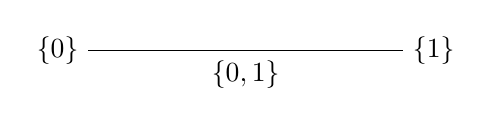
\begin{tikzpicture}
		\draw (-2,0) node[left] {$\{0\}$} node[midway,below] {$\{0,1\}$} -- (2,0) node[right] {$\{1\}$} ;
	\end{tikzpicture}
	\end{center}

\vspace{12pt}

	A \emph{standard 2-simplex}, denoted by $\Delta^2$ is the equilateral triangle.
	\[V_{\Delta^2}=\{0,1,2\}\] \[\mathcal{S}_{\Delta^2}=\{\{0\},\{1\},\{2\},\{0,1\},\{0,2\},\{1,2\},\{0,1,2\}\}\]
	\begin{center}
	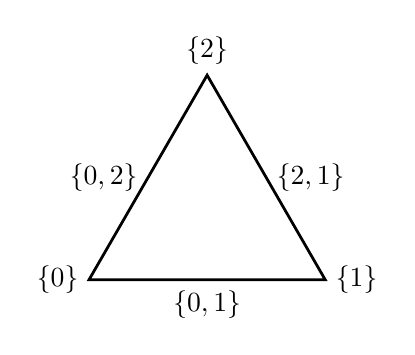
\begin{tikzpicture}
		 \draw [line width=1pt] (0,0) node[left] {$\{0\}$} -- (60:3) node[above] {$\{2\}$}  node[midway,left] {$\{0,2\}$}
		-- (3,0) node[right] {$\{1\}$} node[midway,right] {$\{2,1\}$} -- cycle node[midway,below] {$\{0,1\}$};
	\end{tikzpicture}
	\end{center}

	In general, the \emph{standard $n$-simplex} $\Delta^n$, is $\Delta^n=(V_{\Delta^n},\mathcal{S}_{\Delta^n})$ where
	\[V_{\Delta^n}=\{0,1,\ldots,n\}\] \[\mathcal{S}_{\Delta^n}=\{\alpha:\alpha\subset\{0,\ldots,n\}, \,\alpha\neq\emptyset\}\]
\end{eg}

\vspace{12pt}

\noindent If $X=(V_x,\mathcal{S}_X)$ is a simplicial complex, we now want to pick a field $\mathbb{F}$, usually $\mathbb{Q}$ or $\mathbb{F}_2$ (in this course) and want to produce a sequence of vector 
spaces (over $\mathbb{F}$)

\[C_n(X)_{0\leq n}\]

$C_0(X)$ is the vector space whose basis elements are simply the vertices of the simplicial complex, and this has dimension 0.

\begin{definition}[$k$-simplex of a simplicial complex]
	If $X$ is a simplicial complex then a \emph{$k$-simplex of $X$} is a simplex $\sigma\in\mathcal{S}_X$ such that $|\sigma|=k+1$.
\end{definition}

\noindent $C_k(X)$ is the vector space whose basis elements are the \emph{oriented} $k$-simplices of $X$. If $\{v_0,\ldots,v_n\}$ is an $n$-simplex of $X$, consider the symbols
\[[v_0,v_1,\ldots,v_n]\] such that \[[v_{\rho(0)},v_{\rho(1)},\ldots,v_{\rho(n)}]=\text{sign}(\rho)[v_0,\ldots,v_n]\]

\begin{definition}
	\[\partial_n:C_n(X)\rightarrow C_{n-1}(X)\] is a linear map defined on basis elements as follows;
	\[\partial_n[v_0,\ldots,v_n]=\sum_{r=0}^n(-1)^r[v_o,\ldots,\hat{v_r},\ldots,v_n]\] where $\hat{v_r}$ indincates omission of $v_r$.
\end{definition}

\begin{eg}
	\[\partial_2[0,1,2]=[1,2]-[0,2]+[0,1]\]
	\[\partial_1[v_0,v_2]=[v_1]-[v_0]\]
	\begin{eqnarray*}
		\partial_1\partial_2[0,1,2]&=&\partial_1([1,2]-[0,2]+[0,1]) \\
					&=&([2]-[1])-([2]-[0])+([1]-[0]) \\
					&=&0
	\end{eqnarray*}
\end{eg}

\begin{proposition}[Poincaré lemma]
	Let $X$ be a simplicial complex. Consider \[\partial_r:C_r(X)\rightarrow C_{r-1}(X)\] for $r\geq1$, then \[\partial_{n-1}\partial_n\equiv 0\]
\end{proposition}

\begin{proof}
	\begin{eqnarray*}
		\partial_n[v_0,\ldots,v_n]=\sum_{r=0}^n(-1)^r[v_0,\ldots,\hat{v_r},\ldots,v_n]
	\end{eqnarray*}

	\begin{eqnarray*}
		\partial_{n-1}[v_0,\ldots,\hat{v_r},\ldots,v_n]&=&\sum_{s<r}(-1)^s[v_0,\ldots,\hat{v_s},\ldots,\hat{v_r},\ldots,v_n] \\
									&&+\sum_{s>r}(-1)^{s-1}[v_0\ldots,\hat{v_r},\ldots,\hat{v_s},\ldots,v_n]
	\end{eqnarray*}

	\begin{eqnarray*}
		\partial_{n-1}\partial_n[v_0,\ldots,v_n]&=&\sum_{s<r}(-1)^{r+s}[v_0,\ldots,\hat{v_s},\ldots,\hat{v_r},\ldots,v_n] \\
								&&+\sum_{s>r}(-1)^{r+s-1}[v_0,\ldots,\hat{v_r},\ldots,\hat{v_s},\ldots,v_n] \\
								&=&0
	\end{eqnarray*}
\end{proof}

























\end{document}